%Tipo de documento
\documentclass[a4paper,12pt,twoside]{article} %book, report, letter, beamer


%Paquetes

%Configuracion inicial
\usepackage[utf8]{inputenc}
%\UseRawInputEncoding
\usepackage[spanish]{babel}

%Hipervinculos dinamicos
\usepackage[backref]{hyperref}
%Matematicas
\usepackage{amssymb}
\usepackage{amsmath}
\usepackage{amsbsy}
%Comentarios de varias lineas
\usepackage{comment}
%Insertar imagenes
\usepackage{graphicx}
\graphicspath{ {IMAGENES/} }
%Cuadros de codigo
\usepackage{listings}



% Cuerpo del documento -------------------------------------------------
%Entorno: comando especial que cuenta con parte de incio y de fin.

\begin{document}

%Portada
\begin{titlepage}
\centering

{
\includegraphics[width=0.6\textwidth]{foto_portada.png}\par}
\vspace{1cm}

{\bfseries\LARGE Escuela Técnica Superior de Ingeniería Informática y Telecomunicaciones \par}
\vspace{0.4cm}

{\scshape\Huge Divide y Vencerás \par}
\vspace{0.4cm}

{\itshape\Large Segunda Práctica de Algorítmica \par}
\vspace{0.5cm}

{\itshape\Large Doble Grado en Ingeniería Informática y Matemáticas \par}
\vspace{0.4cm}

{\Large Autores: \par}
{\Large Elena Abreu Fernández \par}
{\Large Antonio Cantillo Molina \par}
{\Large Leandro Jorge Fernández Vega \par}
\vfill

{\Large Abril 2023 \par}

\end{titlepage}

% Crea indice
\tableofcontents
\newpage


\section{Objetivos}


	\begin{itemize}
		\item Conocer en profundidad la implementación de un algoritmo de tipo "Divide y Vencerás".
		\item Saber analizar teórica, empírica e híbridamente un algoritmo recursivo.
		\item Desarrollar una capacidad de pensamiento recursiva además de iterativa.
		\item Aprender a utilizar recursos gráficos como GNUPLOT y aplicar conocimiento estadístico a los análisis.
	\end{itemize}
\newpage


\section{Introducción}

Se plantea la elaboración de un algoritmo de tipo \textit{"Divide y Vencerás"}. Como su propio nombre indica, deberemos descomponer una tarea, a menudo con un tiempo de ejecución elevado, en diversas subtareas y combinar los resultados para ofrecer una solución final, con mejor tiempo de ejecución.\\

Las condiciones necesarias para implementar esta clase de algoritmos correctamente son las siguientes:

\begin{itemize}

	\item El problema tiene que poder descomponerse en subproblemas, más sencillos de resolver que el original.
	\item Los subproblemas deben ser del mismo tipo entre ellos y con el original.
	\item Los subproblemas se resuelven independientemente (casi siempre).
	\item No existe solapamiento entre subproblemas.
	\item Ha de tener sentido combinar las soluciones de los subproblemas para obtener la solución final.

\end{itemize}


\subsection{Datos Técnicos del Computador Utilizado}

\begin{itemize}

	\item Nombre del dispositivo: ASUS LAPTOP-7LR09K87

	\item Procesador: 11th Gen Intel(R) Core(TM) i7-11370H @ 3.30GHz   3.30 GHz

	\item RAM instalada: 16,0 GB (15,7 GB usable)

	\item Tipo de sistema: Sistema operativo de 64 bits.

	\item Arquitectura: x86\_64

	\item Cachés: L1d: 48 KiB (1 instance), L1i: 32 KiB (1 instance), L2: 1.3 MiB (1 instance), L3: 12 MiB (1 instance)

\end{itemize}


\newpage

\subsection{Tipos de Análisis a Realizar}

\subsubsection{Análisis Teórico}

Para determinar a qué orden de eficiencia teórico pertenece un algoritmo, consideramos las siguientes definiciones:

\begin{itemize}

	\item Caso Peor:\\
	\begin{math}
	T(n) \in O(f(n)) \Leftrightarrow \exists K \in \mathbb{R^+} , \exists n_0 \in \mathbb{N} : T(n) \leq K \cdot{f(n)} \ \ \forall n > n_0
	\end{math}
	
	\item Caso Exacto:\\
	\begin{math}	
	T(n) \in \Theta(f(n)) \Leftrightarrow \exists K \in \mathbb{R^+} , \exists n_0 \in \mathbb{N} : T(n) = K \cdot{f(n)} \ \ \forall n > n_0
	\end{math}
	
	\item Caso Mejor:\\
	\begin{math}
	T(n) \in \Omega(f(n)) \Leftrightarrow \exists K \in \mathbb{R^+} , \exists n_0 \in \mathbb{N} : T(n) \geq K \cdot{f(n)} \ \ \forall n > n_0
	\end{math}
	
\end{itemize}

\vspace{1cm}


Para el caso \textit{Divide y Vencerás}, debemos estar preparados para la aparición de ecuaciones recursivas del tipo:\\

$$T(n) = \begin{cases} t(n) \hfill \text{si } n \leq n_o \cr LT(n/b) + G(n) \ \hfill \text{si } n > n_o \end{cases}$$\\

en las cuales:\\

\begin{itemize}

	\item $n_0$ es un umbral para tamaños de problema pequeños.
	\item t(n) es el tiempo de ejecución de un algoritmo adecuado para pequeños tamaños de problema.
	\item L es el número de cada subproblema.
	\item n/b el tamaño de los subproblemas.
	\item G(n) = D(n) + C(n), donde D(n) es el tiempo de dividir el problema en los subproblemas y C(n) el tiempo de combinación de las soluciones de los subproblemas.
\end{itemize}

\newpage
\subsubsection{Análisis Empírico}

El análisis empírico supone la ejecución del algoritmo de ordenación para diferentes tamaños del vector. Para ello, usaremos los siguientes recursos:\\


\begin{itemize}
	\item La biblioteca $<$chrono$>$ y sus funciones para medir tiempos.
	
	\lstset{language=C++}
	\begin{lstlisting}

#include <chrono>
	
high_resolution_clock::time_point t_antes, t_despues;
duration<double> transcurrido;

t_antes = high_resolution_clock::now();

algoritmo(a0,a1,...);

t_despues = high_resolution_clock::now();
transcurrido = 
duration_cast<duration<double>>(t_despues - t_antes);
cout << "el tiempo empleado es " 
<< transcurrido.count() << " s." << endl;
	
	\end{lstlisting}
	
\vspace{1cm}

	\item El siguiente script para automatizar la obtención de resultados para diferentes tamaños:

	\lstset{language=Bash}
	\begin{lstlisting}
#!/bin/bash 
#echo "" >> salida.dat
i=tamanio
while [ "$i" -le tamanio_final ]
do
    ./algoritmo $i >> salida.dat
      i=$(( $i + salto ))
done

	\end{lstlisting}
	
\end{itemize}

\newpage
\subsubsection{Análisis Híbrido}

Consiste en obtener las constantes ocultas de la función del algoritmo. Para ello, utilizamos la herramienta GNUPLOT. Pondremos como ejemplo un algoritmo cuadrático.\\

Primero deberemos introducir la ecuación de la que queremos obtener los coeficientes:\\

\fbox{gnuplot$>$ f(x) = a0*x*x+a1*x+a2}\\

Después le indicaremos a GNUPLOT que realice un ajuste por mínimos cuadrados, donde \textit{salida.dat} es el fichero de datos.\\

\fbox{gnuplot$>$ fit f(x) 'salida.dat' via a0,a1,a2}\\

La parte que más interesa es el apartado \textit{\textbf{Final set of parameters}}, donde se encuentra el valor de los parámetros.\\

Para graficar utilizamos:\\

\fbox{gnuplot$>$ 'salida.dat', f(x) title 'Curva de Ajuste'}\\

Para determinar la bondad del ajuste, podemos utilizar la varianza, aunque el propio análisis teórico y los resultados gráficos nos permiten confirmar que la ecuación parabólica y n-logarítmica representan buenas aproximaciones para los algoritmos a tratar.

\newpage


\section{Problema: Amistad en la Granja}

El problema que se plantea resolver es el siguiente:\\

Un granjero está muy preocupado por el bienestar de su cabaña vacuna. Ha adquirido nuevos terrenos para ampliar el área en que sus vacas pueden pastar y estar relajadas para así producir leche de más calidad. Sabe que las vacas también tienen sus propias preferencias sociales y que, cuando están
libres, cada vaca se acerca a aquella compañera con la que tiene mayor afinidad.\\

Para tener un buen seguimiento de la actividad de cada vaca, cada una tiene un collar equipado con un GPS. De este modo, tiene perfectamente ubicados a todos los ejemplares.\\

Una de las cuestiones de mayor interés es conocer las afinidades entre las vacas. Para cada día que salen del establo al prado se quiere saber cuál es la pareja de vacas que tienen mayor afinidad, es decir, cuál es el par de vacas que están más cerca.


\newpage

\subsection{Explicación}

La resolución del problema la dividiremos en tres partes: generador de casos, algoritmo específico y algoritmo \textit{Divide y Vencerás}.\\

Para ello, se ha pensado como más adecuada la siguiente implementación:\\

\lstset{language=C++}
\begin{lstlisting}
		struct vaca{
		
		    //Identificador
		    int name;
		    //Coordenada x
		    double x;
		    //Coordenada y
		    double y;
		};
	
\end{lstlisting}

\begin{itemize}
	\item \textbf{\textit{name}}: identificador de cada vaca. Se corresponderá con el índice del vector donde están almacenadas todas las vacas.
	\item \textbf{\textit{x}}: Representa la coordenada \textit{x} en el plano donde se sitúa cada vaca.
	\item \textbf{\textit{y}}: Representa la coordenada \textit{y} en el plano donde se sitúa cada vaca.

\end{itemize}

\newpage

\subsection{Generador de Casos}

El término \textit{generador de casos} hace referencia a un programa que establece la situación más adecuada para trabajar.\\

Para ello, generaremos aleatorios en coma flotante que representarán las coordenadas de cada vaca en el plano.\\

Será necesario, posteriormente, procesar los datos del fichero generado para rellenar el vector de vacas sobre el que utilizar el algoritmo.



\lstset{language=C++}
\begin{lstlisting}

#include <iostream>
#include <fstream>
#include <cmath>
#include <random>
#include <time.h>
#include <chrono>

using namespace std;

int main(int argc, char *argv[]) {

    if (argc > 3) exit(-1);
    else {
        const int MIN = 0, MAX = 5;
        std::random_device rd;
        std::default_random_engine eng(rd());
        std::uniform_real_distribution<double> distr(MIN, MAX);


        // Tomamos numero de vacas y nombre del fichero 
        //del caso generado.

        int numero_vacas = stoi(argv[1]);
        string fichero = argv[2];

        // Relleno de fichero.

        ofstream salida;
        salida.open(fichero);

        salida << numero_vacas << endl;
        for (int i = 0; i < numero_vacas; i++) {
            salida << i << " " << distr(eng) << " " << distr(eng) 
            << endl;
        }

        // Cerramos fichero

        salida.close();
    }

    return 0;
}
\end{lstlisting}

\newpage

\subsection{Algoritmo Específico}

El objetivo de este algoritmo es la obtención de soluciones del problema, para tamaños menores que un umbral determinado.\\

La implementación de este algoritmo es la siguiente:

\lstset{language=C++}
\begin{lstlisting}

double distancia(vaca vaca_1, vaca vaca_2) {

    return sqrt(pow(vaca_1.x-vaca_2.x,2) 
    	+ pow(vaca_1.y-vaca_2.y,2));		//O(1)
}


pair<int,int> AlgoritmoEspecifico(vector <vaca> vacas,int inicio, 
	int final){
    
    double min= distancia(vacas[inicio],vacas[inicio+1]);
    pair<int,int> salida(inicio, inicio+1);

    for(int i=inicio; i<final; i++){	//O(n)
        for(int j=i+1;j<final; j++){	//O(n)
            double posible_min=distancia(vacas[i],vacas[j]);
            if (posible_min < min){
                min= posible_min;
                salida.first=i;
                salida.second=j;
            }
        }
    }

    return salida;
}

\end{lstlisting}

\newpage

\subsubsection{Análisis Teórico}

Claramente $T(n) \in O(n^2)$, pues:\\

Considerando el inicio en $i=0$ (caso peor) hasta $final=n$:\\

$\sum_{i=0}^{n-1} \sum_{j=i+1}^{n-1} 1 = 
\sum_{i=0}^{n-1} (n-1)-(i+1)+1 =
\sum_{i=0}^{n-1} n-i-1 =\\
n^2 - n - \sum_{i=0}^{n-1} i =
n^2 - n - \frac{(n-1)(n-1+1)}{2}= \frac{n^2-n}{2}$



\subsubsection{Análisis Empírico}


\begin{table}[h]
	\begin{center}
		\begin{tabular}{|c|c|}
		\hline
		Tamaño & Tiempo \\
		\hline
		500 & 0.00978403 \\
		1000 & 0.0247866 \\
		1500 & 0.0490347 \\
		2000 & 0.0845467 \\
		2500 & 0.134698 \\
		3000 & 0.189079 \\
		3500 & 0.260813 \\
		4000 & 0.340241 \\
		4500 & 0.463539 \\
		5000 & 0.562085 \\
		5500 & 0.658605 \\
		6000 & 0.772989 \\
		6500 & 0.936878 \\
		7000 & 1.11724 \\
		7500 & 1.21901 \\
		8000 & 1.36652 \\
		8500 & 1.52628 \\
		9000 & 1.72578 \\
		9500 & 1.90376 \\
		10000 & 2.12881 \\
		10500 & 2.40041 \\
		11000 & 2.66086 \\
		11500 & 3.15399 \\
		12000 & 3.33043 \\
		12500 & 3.45203 \\
		\hline
		\end{tabular}
	\end{center}
	\caption{Algoritmo Especifico}
\end{table}

\newpage


\subsubsection{Análisis Híbrido}

\begin{figure}[h]
  \begin{center}
  
  	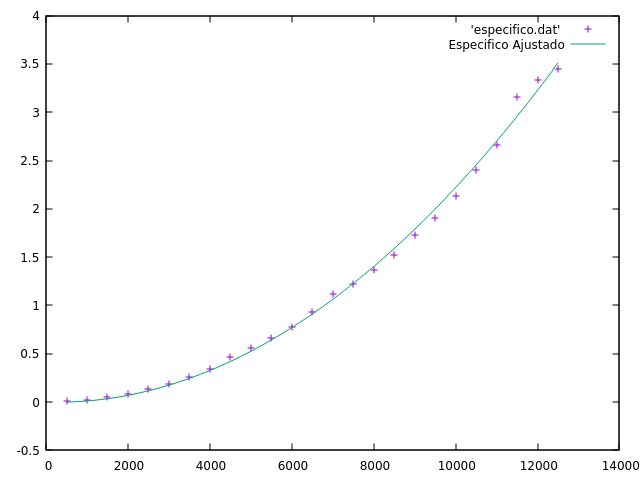
\includegraphics[scale=0.7]{especifico_ajustado.png}
  	\caption{Promedio: Específico ajustado.}
  	
  \end{center}
\end{figure}


El análisis teórico nos permite comprobar que la curva de ajuste es una parábola de ecuación:\\

$T(n) = 2.33791 \cdot{10^{-8}} n^2 -1.18345 \cdot{10^{-5}} n + 1.0461  \cdot{10^{-7}} $\\

con una varianza residual $Var_{res} =0.00419557$, con lo cual es fiable el ajuste.

\newpage

\subsection{Algoritmo \textit{Divide y Vencerás}}


\paragraph{Idea}
Para la elaboración del algoritmo \textit{Divide y Vencerás}, ordenaremos primero las vacas por la coordenada \textit{x} mediante un algoritmo de ordenación (a poder ser n-logarítmico para no alterar la eficiencia). Esto nos permitirá dividir el plano en dos mitades, y facilitar las comparaciones mediante métodos explicados posteriormente.


\lstset{language=C++}
\begin{lstlisting}

const int UMBRAL_VACAS;


pair<int,int> DyV(vaca vacas[], int n){

    quicksort(vacas,n);	//Algoritmo de ordenacion, 
    			//a poder ser n-logaritmico

    return DyV_lims(vacas,0,n);
}

//----------------------------------------------------------



pair<int,int> DyV_lims(vaca vacas[], int inicio, int final) {

    pair<int,int> output1, output2, output;

    if (final-inicio <= UMBRAL_VACAS) 
    output=AlgoritmoEspecifico(vacas, inicio, final);

    else {
        int medio=(inicio+final)/2;
        output1=DyV_lims(vacas, inicio, medio);
        output2=DyV_lims(vacas,medio, final);

        if (distancia(vacas[output1.first],vacas[output1.second]) 
        < distancia(vacas[output2.first],vacas[output2.second]))
            output=output1;
        else output=output2;

        
        double dist_min =
        distancia(vacas[output.first],vacas[output.second]);


        for (int i=inicio; i<medio; i++){
            //Pertenecer al rectangulo.
            if(abs(vacas[i].x - vacas[medio].x) < dist_min) {

                for (int j=medio; j<final; j++){
                    if(abs(vacas[j].x - vacas[medio].x) 
                    < dist_min){

                        double dist= distancia(vacas[i],vacas[j]);
                        //Comparamos cada punto de una mitad del
                        //rectangulo con cada uno de la otra.
                        if(dist < dist_min){
                            dist_min=dist;
                            output.first=i;
                            output.second=j;
                        }
                    }
                }
            }
        }
    }

    return output;
}

//----------------------------------------------------------


\end{lstlisting}

\newpage

\subsubsection{Análisis Teórico}


Debemos tener claro que la parte recursiva es de la forma $2T(n/2)$. A esto deberemos añadirle el tiempo de dividir en subcasos y la combinación de soluciones. Para ver esto recurrimos al siguiente teorema:

\paragraph{Teorema}

Sea P el conjunto de todos los puntos y P' son todos los puntos que se encuentran a una distancia menor a dmin=distancia mínima de l=línea divisoria del plano. Si P[i] y P[j] (i $<$ j) son la dupla mas cercana de puntos en P' y la distancia entre ellos es menor que dmin, entonces $j-i <= 7$.

\paragraph{Demostración}

Supongamos que P'[i] y P'[j] son los puntos más cercanos en P' con una distancia menor a dmin. Por ser su distancia menor que dmin, entonces $|$ P'[i].y - P'[j].y $|$ $<$ dmin, esto nos indica que ambos puntos se encuentran dentro de un rectángulo de ancho 2dmin y alto dmin, centrado en l. Ahora, dividamos este rectángulo en ocho cuadrados del mismo tamaño de lado dmin/2, por lo que la longitud de la diagonal de cada cuadrado (Teorema de Pitágoras) esta dada por:\\

$\sqrt{\frac{dmin^2}{4}+\frac{dmin^2}{4}}= \frac{dmin}{\sqrt{2}} < dmin$\\

Como cada cuadrado se encuentra completamente a un lado de l, ningún cuadrado puede contener dos puntos de P, ya que si los tuviera, entonces ambos puntos estarían a una distancia menor que dmin y dmin no sería entonces la distancia mínima a ambos lados de l. Por lo tanto puede haber a lo sumo 8 puntos de P' en este rectángulo y por lo tanto $j-i <= 7$.\\

Por tanto, la ecuación de recurrencia para el algoritmo es $2T(n/2) + O(n)$. 

Partiendo de una ecuación recurrente de la forma $LT(n/b) + G(n)$, sabemos que si $G(n) \in O(n^k) \Rightarrow T(n) \in O(n^k \log{n})$ si 
$L=b^k$

Finalmente, deducimos que $T(n) \in O(n \log{n})$, pues $b=2, L=2, k=1$.
\newpage

\subsubsection{Análisis Empírico}

\begin{table}[h]
	\begin{center}
		\begin{tabular}{|c|c|}
		\hline
		Tamaño & Tiempo \\
		\hline
		500 & 0.000696375 \\
		1000 & 0.0015033 \\
		1500 & 0.00174132 \\
		2000 & 0.00160477 \\
		2500 & 0.00184455 \\
		3000 & 0.00211836 \\
		3500 & 0.00282064 \\
		4000 & 0.00294878 \\
		4500 & 0.00343699 \\
		5000 & 0.00392889 \\
		5500 & 0.00384519 \\
		6000 & 0.00477511 \\
		6500 & 0.00555737 \\
		7000 & 0.00575071 \\
		7500 & 0.00681028 \\
		8000 & 0.00674871 \\
		8500 & 0.00738019 \\
		9000 & 0.00792721 \\
		9500 & 0.00839595 \\
		10000 & 0.00933103 \\
		10500 & 0.00958622 \\ 
		11000 & 0.0097171 \\
		11500 & 0.0107547 \\
		12000 & 0.0154529 \\
		12500 & 0.0147265 \\
		\hline
		\end{tabular}
	\end{center}
	\caption{Algoritmo DyV}
\end{table}

\newpage

\subsubsection{Análisis Híbrido}

\begin{figure}[h]
  \begin{center}
  
  	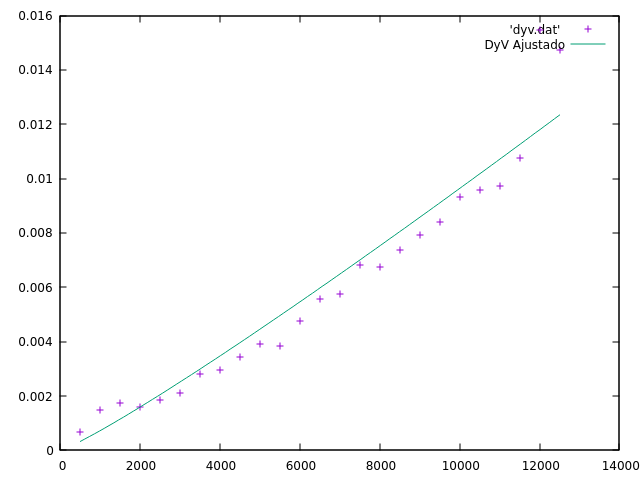
\includegraphics[scale=0.7]{dyv_ajustado.png}
  	\caption{Promedio: DyV ajustado.}
  	
  \end{center}
\end{figure}

El análisis teórico nos permite determinar que la curva que mejor se ajusta es una n-logarítmica de ecuación:\\

$T(n)= 1.0461 \cdot{10^{-7}} n \log{n}$\\

con una varianza residual $Var_{res} =1.13885 \cdot {10^{-6}}$, con lo cual es fiable el ajuste.

\newpage


\subsection{Cálculo de Umbrales}

En esta sección determinaremos cuál es el umbral bajo el que aplicar el algoritmo específico.


\subsubsection{Umbral Teórico}

Para calcular el umbral teórico, debemos ver primero, aproximadamente, cuántas operaciones totales se llevan a cabo:

\begin{itemize}
	\item Función distancia: 5
	\item Algoritmo Específico: $6 + \frac{9}{2} n(n-1)$
	\item Algoritmo \textit{Divide y Vencerás}: $15+35n +2T(n/2)$
\end{itemize}

Para el cálculo teórico del umbral debemos resolver la ecuación:\\

$T(n)=t(n) \Leftrightarrow  Lt(n/b) + G(n) = t(n) \Leftrightarrow \\
6 + \frac{9}{2} n(n-1) = 2(6 + \frac{9}{2} \frac{n}{2}(\frac{n}{2}-1)) +15 +35n \Leftrightarrow n_0 \approx 16
$

\subsubsection{Umbral Óptimo}

Para el cálculo del umbral óptimo, debemos igualar las ecuaciones ajustadas del algoritmo específico y el \textit{Divide y Vencerás}:\\

$T_1(n) = T_2(n) \Leftrightarrow \\
2.33791 \cdot{10^{-8}} n^2 -1.18345 \cdot{10^{-5}} n + 1.0461  \cdot{10^{-7}} = 1.0461 \cdot{10^{-7}} n \log{n}$\\

Esta ecuación no tiene solución, por lo que no hay umbral. Deberemos ver a través del umbral de tanteo qué ocurre con las variaciones del umbral.\\

\newpage

\subsubsection{Umbral de Tanteo}

La siguiente gráfica ilustra cómo un umbral cada vez menor supone mejores tiempos de ejecución para el algoritmo, pues aunque para un tramo inicial de valores la diferencia no es tan significativa, a largo plazo es necesario tenerla en consideración. Podríamos decir que, en caso de poner un umbral, el óptimo sería de alrededor 4 vacas.

\begin{figure}[h]
  \begin{center}
  
  	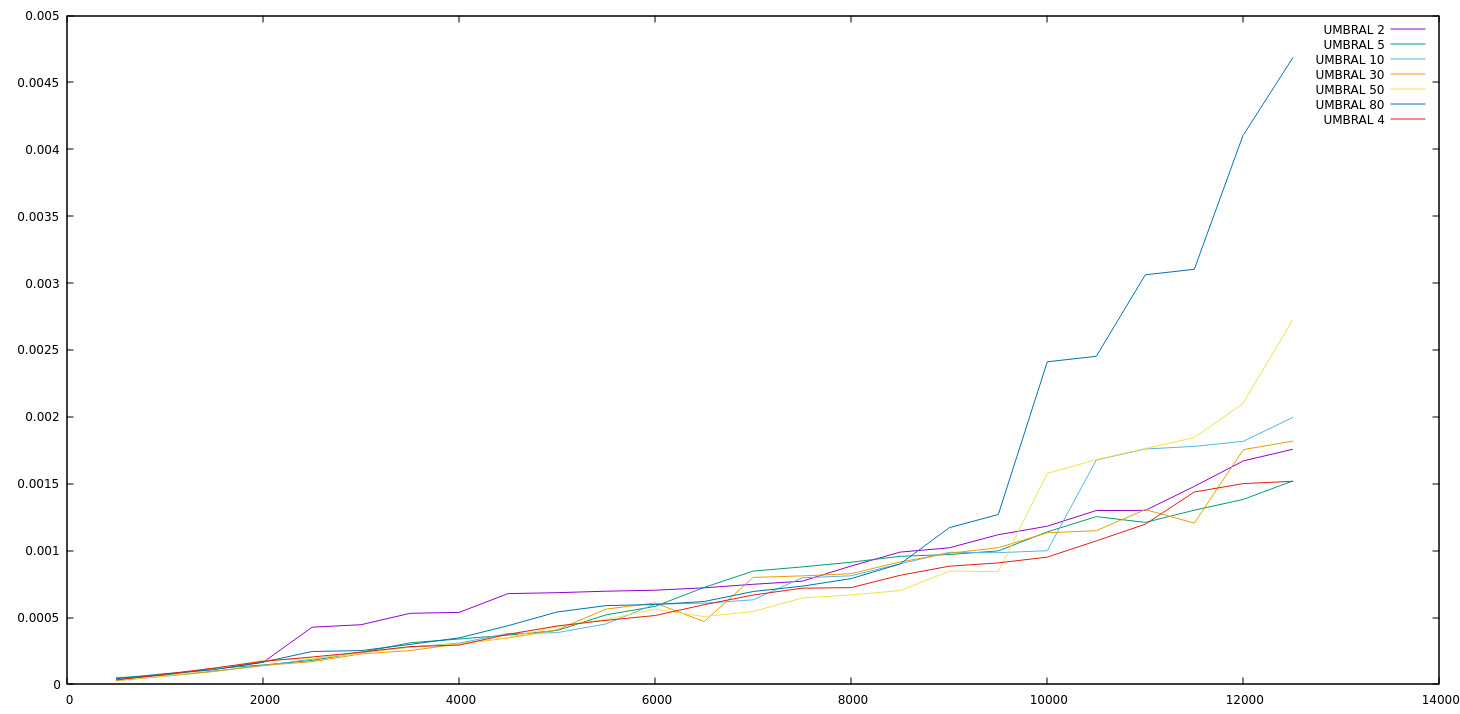
\includegraphics[scale=0.3]{comparacion_umbrales.jpeg}
  	\caption{Comparación de umbrales.}
  	
  \end{center}
\end{figure}


Por tanto, concluimos que el algoritmo \textit{Divide y Vencerás} mejora en su totalidad, o prácticamente en su totalidad, al específico.

\newpage

\subsubsection{Comparaciones}

En esta sección ofrecemos una comparativa final de los tiempos de ejecución variando umbrales.\\

\begin{figure}[h]
  \begin{center}
  
  	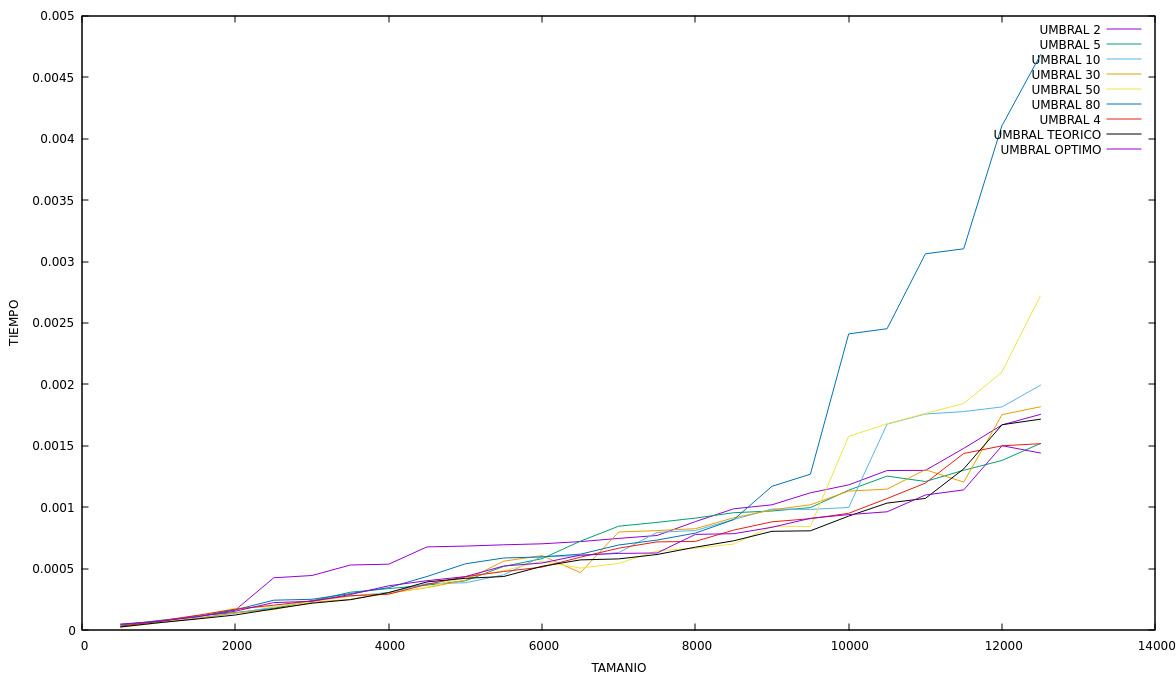
\includegraphics[scale=0.35]{comparacion.jpeg}
  	\caption{Comparación de todos los umbrales.}
  	
  \end{center}
\end{figure}

\newpage

\section{Conclusiones} 

\begin{itemize}
	\item La importancia del uso de la recursividad en la reducción del tiempo de ejecución.
	\item La necesidad de controlar la recursividad para evitar llamadas excesivas que acaben en colapsos de la pila y otros problemas.
	\item La versatilidad que ofrece la técnica \textit{Divide y Vencerás} para la resolución de problemas.
	\item La necesidad de ampliar el conocimiento algorítmico para la resolución de cualquier problema.
	\item La variación que puede existir entre los cálculos teóricos y empíricos debido a las características de cada dispositivo y el grado de precisión que, en cada circusntancia, es posible tomar.
	

\end{itemize}



\end{document}